\documentclass[tikz,border=2pt]{standalone}
\usepackage{tikz}
\usepackage{helvet}
\usetikzlibrary{arrows.meta,positioning}

\begin{document}
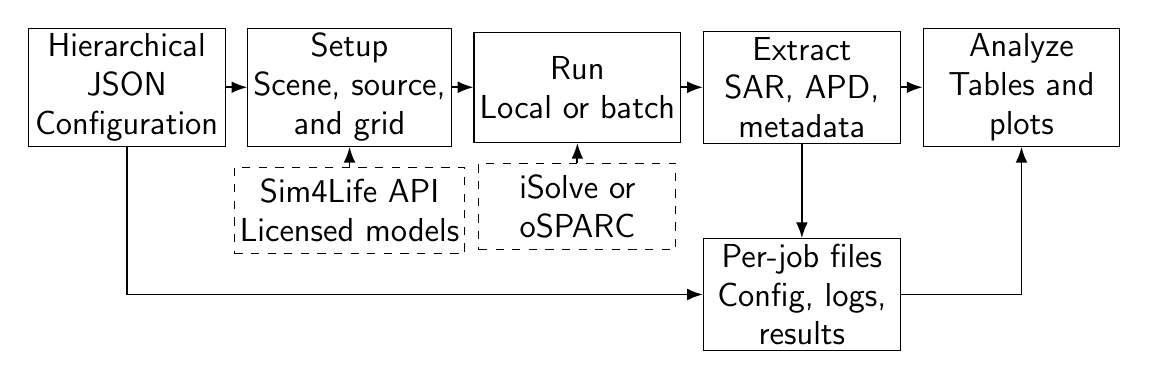
\begin{tikzpicture}[
  font=\sffamily\large,
  box/.style={draw=black, rectangle, minimum width=25mm, minimum height=14mm,
              align=center, inner sep=2pt},
  ext/.style={draw=black, dashed, rectangle, minimum width=25mm,
              minimum height=11mm, align=center, inner sep=2pt},
  arrow/.style={-{Latex[length=2mm]}, line width=0.65pt},
]
  \node[box] (config) {Hierarchical\\JSON\\Configuration};
  \node[box, right=2.75mm of config] (setup) {Setup\\Scene, source,\\and grid};
  \node[box, right=2.75mm of setup] (run) {Run\\Local or batch};
  \node[box, right=2.75mm of run] (extract) {Extract\\SAR, APD,\\metadata};
  \node[box, right=2.75mm of extract] (analyse) {Analyze\\Tables and\\plots};

  \draw[arrow] (config) -- (setup);
  \draw[arrow] (setup) -- (run);
  \draw[arrow] (run) -- (extract);
  \draw[arrow] (extract) -- (analyse);

  \node[ext, below=2.5mm of setup] (models) {Sim4Life API\\Licensed models};
  \node[ext, below=2.5mm of run] (solvers) {iSolve or\\oSPARC};
  \draw[arrow] (models) -- (setup);
  \draw[arrow] (solvers) -- (run);

  \node[box, below=12mm of extract] (record) {Per-job files\\Config, logs,\\results};
  \draw[arrow] (config.south) |- (record.west);
  \draw[arrow] (extract) -- (record);
  \draw[arrow] (record.east) -| (analyse.south);
\end{tikzpicture}
\end{document}
